\documentclass{article}
\usepackage{amsmath}
\usepackage{amsfonts}
\usepackage{amssymb}
\usepackage{enumitem}
\usepackage{tikz}
\usepackage{mathtools}

\usetikzlibrary{arrows}

\title{CSC 226 - Assignment 4 - Theory}
\date{April 2017}
\author{Daniel Frankcom}

\begin{document}
	\pagenumbering{gobble}
	\maketitle
	\setlength{\parindent}{0pt}
	\newcommand{\forceindent}{\leavevmode{\parindent=72pt\indent}}
	\newpage
	\pagenumbering{arabic}
	
	\begin{enumerate}
		\item \quad
		\newline
		\begin{center}
			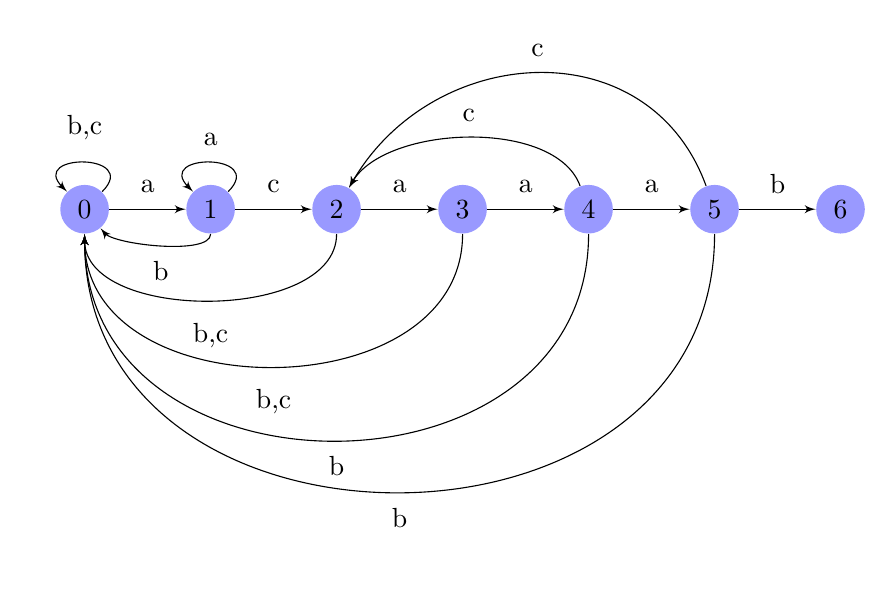
\begin{tikzpicture}
			[scale=.8,auto=left,every node/.style={circle,fill=blue!40}, edge/.style={->,> = latex'}]
			\node (n0) at (0,0)  {0};
			\node (n1) at (2,0)  {1};
			\node (n2) at (4,0)  {2};
			\node (n3) at (6,0)  {3};
			\node (n4) at (8,0)  {4};
			\node (n5) at (10,0)  {5};
			\node (n6) at (12,0)  {6};
			
			\draw[edge] (n0) to node [above, fill=none] {a} (n1);
			\draw[edge] (n1) to node [above, fill=none] {c} (n2);
			\draw[edge] (n2) to node [above, fill=none] {a} (n3);
			\draw[edge] (n3) to node [above, fill=none] {a} (n4);
			\draw[edge] (n4) to node [above, fill=none] {a} (n5);
			\draw[edge] (n5) to node [above, fill=none] {b} (n6);
			
			\draw[edge] (n0) to [out=45,in=135,looseness=4] node [above, fill=none] {b,c} (n0);
			\draw[edge] (n1) to [out=270,in=310,looseness=0.5] node [below, fill=none] {b} (n0);
			\draw[edge] (n1) to [out=45,in=135,looseness=4] node [above, fill=none] {a} (n1);
			\draw[edge] (n2) to [out=270,in=270,looseness=0.9] node [below, fill=none] {b,c} (n0);
			\draw[edge] (n3) to [out=270,in=270,looseness=1.2] node [below, fill=none] {b,c} (n0);
			\draw[edge] (n4) to [out=270,in=270,looseness=1.4] node [below, fill=none] {b} (n0);
			\draw[edge] (n4) to [out=110,in=60,looseness=0.8] node [above, fill=none] {c} (n2);
			\draw[edge] (n5) to [out=270,in=270,looseness=1.4] node [below, fill=none] {b} (n0);
			\draw[edge] (n5) to [out=110,in=60,looseness=1.2] node [above, fill=none] {c} (n2);
			
			\end{tikzpicture}
		\end{center}
		
		\item Any example where both the search and pattern strings are entirely made up of one character performs poorly, as the algorithm is not able to skip forward when comparing characters.
		\newline Search string:\hspace{10pt} "AAAAAAAAAAAAAAAA"
		\newline Pattern string:\quad "AA"
		
		\item
		\begin{enumerate}
			\item This statement is false. A counterexample for this is the following:
			\newline
			\begin{center}
				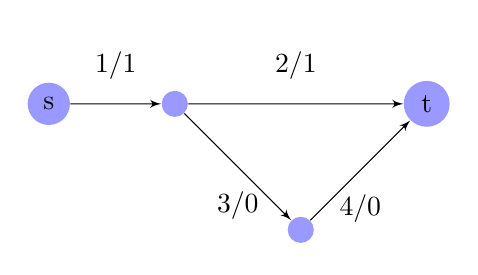
\begin{tikzpicture}
				[scale=.8,auto=left,every node/.style={circle,fill=blue!40}, edge/.style={->,> = latex'}]
				\node (n0) at (0,2)  {s};
				\node (n1) at (2,2)  {};
				\node (n2) at (4,0)  {};
				\node (n3) at (6,2)  {t};
	
				\draw[edge] (n0) to node [above, fill=none] {1/1} (n1);
				\draw[edge] (n1) to node [above, fill=none] {2/1} (n3);
				\draw[edge] (n1) to node [below, fill=none] {3/0} (n2);
				\draw[edge] (n2) to node [below, fill=none] {4/0} (n3);			
				\end{tikzpicture}
				
				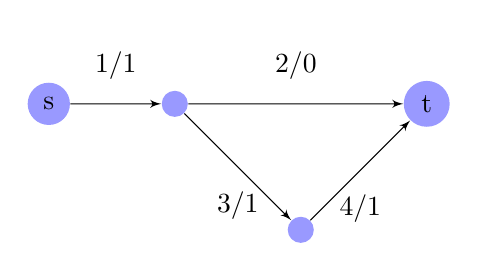
\begin{tikzpicture}
				[scale=.8,auto=left,every node/.style={circle,fill=blue!40}, edge/.style={->,> = latex'}]
				\node (n0) at (0,2)  {s};
				\node (n1) at (2,2)  {};
				\node (n2) at (4,0)  {};
				\node (n3) at (6,2)  {t};
				
				\draw[edge] (n0) to node [above, fill=none] {1/1} (n1);
				\draw[edge] (n1) to node [above, fill=none] {2/0} (n3);
				\draw[edge] (n1) to node [below, fill=none] {3/1} (n2);
				\draw[edge] (n2) to node [below, fill=none] {4/1} (n3);			
				\end{tikzpicture}
			\end{center}
			
			\item This is true. For any given maximum flow with a positive flow cycle, we can reduce the flow of each edge in the cycle so that at least one of the edges has flow 0, while maintaining the overall flow of the graph.
			
			\item This is true. Since all edge capacities are increased by the same amount, the hierarchy of edges remains the same. Since the algorithm to find the min cut inspects the relative order of the edges, if this remains unchanged, then the min cut will also remain unchanged.
		\end{enumerate}
		
		\item This problem is tough, as we cannot simply apply the node capacity to each of the outgoing edges, as multiple edges would cause the node to gain more overall output capacity.
		\newline
		\newline An example of a problem graph is the following:
		\begin{center}
			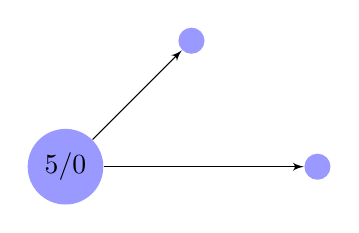
\begin{tikzpicture}
			[scale=.8,auto=left,every node/.style={circle,fill=blue!40}, edge/.style={->,> = latex'}]
			\node (n0) at (0,0)  {5/0};
			\node (n1) at (2,2)  {};
			\node (n2) at (4,0)  {};
			
			\draw[edge] (n0) to node [above, fill=none] {} (n1);
			\draw[edge] (n0) to node [above, fill=none] {} (n2);
			\end{tikzpicture}
		\end{center}
		
		We can deal with this issue by adding more nodes to the graph. Specifically, we will add a node to accept incoming edges, which will then point to our original node.
		
		\begin{center}
			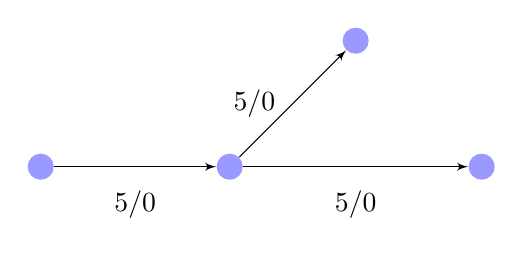
\begin{tikzpicture}
			[scale=.8,auto=left,every node/.style={circle,fill=blue!40}, edge/.style={->,> = latex'}]
			\node (n0) at (3,0)  {};
			\node (n1) at (5,2)  {};
			\node (n2) at (7,0)  {};
			\node (n3) at (0,0)  {};
			
			\draw[edge] (n0) to node [left, fill=none] {5/0} (n1);
			\draw[edge] (n0) to node [below, fill=none] {5/0} (n2);
			\draw[edge] (n3) to node [below, fill=none] {5/0} (n0);
			\end{tikzpicture}
		\end{center}
		
		In this manner, the total flow through the original node will be limited by the incoming node. The outgoing edges from our original node will have capacity $c_v$. This will ensure that if all of the flow needs to go through a single edge, it still can.
		
		
		
		\item This problem can be simply reduced to a max flow problem by creating a residual graph where each edge in $G$ is represented as an edge with flow 1. In this manner, when an arbitrary path is chosen during the computation of the max flow, the 1 unit of flow will no longer be available, so we will not choose another path which repeats the same edge.
		
	\end{enumerate}
\end{document}